\documentclass[11pt]{article} 
\usepackage{amsmath}
\usepackage{amsfonts}
\usepackage{amssymb}
\usepackage{geometry}
\geometry{a4paper, margin=1in}
\usepackage{graphicx}
\usepackage[hidelinks]{hyperref}
\usepackage{amsthm}
\usepackage{tikz}
\usepackage{subcaption}
\usetikzlibrary{positioning}
\usepackage{pgfplots} 
\usepackage[ruled,vlined]{algorithm2e} 
\usepackage{dsfont}
\usepackage{graphicx}
\usepackage{mathdesign}
\usepackage{float}
\usepackage{todonotes} 
\usepackage{empheq}
\usepackage{array}
\usepackage[ruled,vlined]{algorithm2e} 
\usepackage[many]{tcolorbox}    	% for COLORED BOXES (tikz and xcolor included)



\newtcolorbox{boxA}{
    fontupper = \bf,
    boxrule = 1.5pt,
    colframe = black % frame color
}


\setlength{\parindent}{0pt}
\numberwithin{equation}{section}


\newcommand\mycommfont[1]{\footnotesize\ttfamily\textcolor{blue}{#1}}
\newcommand\defeq{\stackrel{\mathclap{\normalfont\mbox{def}}}{=}}
\SetCommentSty{mycommfont}

\DeclareMathOperator*{\argmax}{argmax}
\DeclareMathOperator*{\argmin}{argmin}



\newtheoremstyle{boldStyle}%                % Name
  {}%                                     % Space above
  {}%                                     % Space below
  {\itshape}%                                     % Body font
  {}%                                     % Indent amount
  {\bfseries}%                            % Theorem head font
  {}%                                    % Punctuation after theorem head
  {\newline}                              % Space after theorem head, new line
  {\thmname{#1}\thmnumber{ #2}\thmnote{ (#3)}}%                                     % Theorem head spec (can be left empty, meaning `normal')


\theoremstyle{boldStyle}
\newtheorem{theorem}{Theorem}[section]
\newtheorem{lemma}{Lemma}[section]
\newtheorem{definition}{Definition}[section]
\newtheorem{corollary}{Corollary}[section]
\newtheorem{claim}{claim}[section]
\newtheorem{example}{Example}[section]


\newtheorem*{claim*}{Claim}
\newtheorem*{lemma*}{Lemma}
\newtheorem*{corollary*}{Corollary}
\newtheorem*{remark*}{Remark}
\newtheorem*{example*}{Example}
\newtheorem*{examples*}{Examples}
\newtheorem*{definition*}{Definition}



\title{
    \Huge Transactions of the Fourth Prague Conference\\
    \Large on Information Theory, Statistical Decision Functions, Random Processes \\
    \large Held at Prague, from August 31 to September 11, 1965 \\
    \vspace{10pt}
    \normalsize Behaviour of Sequential Predictors of Binary Sequences
}

\author{T. M. Cover}
\date{Published by the Publishing House of the Czechoslovak Academy of Sciences, Prague 1967}



\begin{document}
\maketitle

% * * * * * * * * * * * * * * * * * * * * * * * * 
% * * * * * * * * * * * * * * * * * * * * * * * * 
% * * * * * * * * * * * * * * * * * * * * * * * * 
% * * * * * * * * * * * * * * * * * * * * * * * * 
% * * * * * * * * * * * * * * * * * * * * * * * * 
% * * * * * * * * * * * * * * * * * * * * * * * * 
% * * * * * * * * * * * * * * * * * * * * * * * * 
% * * * * * * * * * * * * * * * * * * * * * * * * 
% * * * * * * * * * * * * * * * * * * * * * * * * 
% * * * * * * * * * * * * * * * * * * * * * * * * 
% * * * * * * * * * * * * * * * * * * * * * * * * 
% * * * * * * * * * * * * * * * * * * * * * * * * 
% * * * * * * * * * * * * * * * * * * * * * * * * 
% * * * * * * * * * * * * * * * * * * * * * * * * 
% * * * * * * * * * * * * * * * * * * * * * * * * 
% * * * * * * * * * * * * * * * * * * * * * * * * 
% * * * * * * * * * * * * * * * * * * * * * * * * 
% * * * * * * * * * * * * * * * * * * * * * * * * 
% * * * * * * * * * * * * * * * * * * * * * * * * 
\section{Introduction}


% * * * * * * * * * * * * * * * * * * * * * * * * 
% * * * * * * * * * * * * * * * * * * * * * * * * 
% * * * * * * * * * * * * * * * * * * * * * * * * 
% * * * * * * * * * * * * * * * * * * * * * * * * 
% * * * * * * * * * * * * * * * * * * * * * * * * 
% * * * * * * * * * * * * * * * * * * * * * * * * 
% * * * * * * * * * * * * * * * * * * * * * * * * 
% * * * * * * * * * * * * * * * * * * * * * * * * 
% * * * * * * * * * * * * * * * * * * * * * * * * 
% * * * * * * * * * * * * * * * * * * * * * * * * 
% * * * * * * * * * * * * * * * * * * * * * * * * 
% * * * * * * * * * * * * * * * * * * * * * * * * 
% * * * * * * * * * * * * * * * * * * * * * * * * 
% * * * * * * * * * * * * * * * * * * * * * * * * 
% * * * * * * * * * * * * * * * * * * * * * * * * 
% * * * * * * * * * * * * * * * * * * * * * * * * 
% * * * * * * * * * * * * * * * * * * * * * * * * 
% * * * * * * * * * * * * * * * * * * * * * * * * 
% * * * * * * * * * * * * * * * * * * * * * * * * 
\section{Deterministic Predictors}

Consider the set of $2^n$ sequences $\Theta = (\Theta_1, \Theta_2, \ldots, \Theta_{n}) \in \{0, 1\}^n$.

At stage $k$, after the observation $\Theta_1, \Theta_2, \ldots, \Theta_{k-1}$, the prediction 1 or 0 will be made with probability $p_k$ and $1-p_k$ respectively.

\begin{definition}[Sequential Predictor]
    A sequential predictor on $\{0, 1\}^n$ will be completely specified by the set of functions 
    \[
        p_1, p_2(\Theta_1), p_3(\Theta_1, \Theta_2), \ldots, p_n(\Theta_1, \Theta_2, \ldots, \Theta_{n-1})
    \]
    taking values in $[0, 1]$.
    \begin{itemize}
        \item If the $p_i$s are restricted to $\{0, 1\}$, the predictor is called a \textbf{deterministic predictor}.
        \item If the $p_i$s are independent of the $\Theta$s, the predictor is called a \textbf{memoryless predictor}.
        \item If the $p_i$s are also independent of $i$, the predictor is called a \textbf{constant/time invariant predictor}.
    \end{itemize}
\end{definition}

Let $\delta = (\delta_1, \delta_2, \ldots, \delta_n) \in \{0, 1\}^n$ be the sequence of R.V.s resulting from the predictor $p = (p_1, p_2, \ldots, p_n)$ and the sequence $\Theta \in \{0, 1\}^n$.

Then the empirical average score (the fraction of correct predictions) is given by

\begin{align}
    s = \frac{1}{n} \sum_{i=1}^{n} [\delta_i \Theta_i + (1 - \delta_i)(1 - \Theta_i)]
\end{align}

and the expected empirical average score is given by

\begin{align}
    \bar{s} = \mathbb{E}_{p}(s) =  \frac{1}{n} \sum_{i=1}^{n} [p_i \Theta_i + (1 - p_i)(1 - \Theta_i)] 
\end{align}

\begin{theorem}
    Any sequential deterministic predicator attains a score of $\frac{k}{n}$ on precisely $\binom{n}{k}$ sequences in $\{0, 1\}^n$ where $k \in [n]$.
    For any deterministic predictor, there exists a sequence upon which a score of 0 is attained.
\end{theorem}



% * * * * * * * * * * * * * * * * * * * * * * * * 
% * * * * * * * * * * * * * * * * * * * * * * * * 
% * * * * * * * * * * * * * * * * * * * * * * * * 
% * * * * * * * * * * * * * * * * * * * * * * * * 
% * * * * * * * * * * * * * * * * * * * * * * * * 
% * * * * * * * * * * * * * * * * * * * * * * * * 
% * * * * * * * * * * * * * * * * * * * * * * * * 
% * * * * * * * * * * * * * * * * * * * * * * * * 
% * * * * * * * * * * * * * * * * * * * * * * * * 
% * * * * * * * * * * * * * * * * * * * * * * * * 
% * * * * * * * * * * * * * * * * * * * * * * * * 
% * * * * * * * * * * * * * * * * * * * * * * * * 
% * * * * * * * * * * * * * * * * * * * * * * * * 
% * * * * * * * * * * * * * * * * * * * * * * * * 
% * * * * * * * * * * * * * * * * * * * * * * * * 
% * * * * * * * * * * * * * * * * * * * * * * * * 
% * * * * * * * * * * * * * * * * * * * * * * * * 
% * * * * * * * * * * * * * * * * * * * * * * * * 
% * * * * * * * * * * * * * * * * * * * * * * * * 
\section{Sequential Betting Systems}

% * * * * * * * * * * * * * * * * * * * * * * * * 
% * * * * * * * * * * * * * * * * * * * * * * * * 
% * * * * * * * * * * * * * * * * * * * * * * * * 
% * * * * * * * * * * * * * * * * * * * * * * * * 
% * * * * * * * * * * * * * * * * * * * * * * * * 
\subsection{Achievable Winnings in Sequential Betting}

A series of \(n\) bets \(b = (b_1, b_2, \ldots, b_n)\) is made by a gambler on the outcomes of a sequence \(\Theta = (\Theta_1, \Theta_2, \ldots, \Theta_n) \in \{0, 1\}^n\).
The gambler's net gain at bet \(k\) is \(b_k\) if \(\Theta_k = 1\) and \(-b_k\) if \(\Theta_k = 0\). Hence, his net winnings \(w(\Theta)\) using strategy \(b\) against sequence \(\Theta\) is
\begin{align} \label{eq:3.1}
    w(\Theta) = \sum_{k=1}^n \left(b_k \Theta_k - b_k(1 - \Theta_k)\right) = \sum_{k=1}^n b_k(2\Theta_k - 1),
\end{align}

where, in general, \(b_k\) will be a real valued function of \(\Theta\).

\medbreak

Notice that a gambler may win any preassigned amount \(w(\Theta)\) if \(\Theta\) is known a priori. For example, any \(w\) could be achieved with the betting system
\begin{equation} \label{eq:3.2}
    \begin{aligned}
        b_1 &= w(\Theta) \Theta_1 - w(\Theta)(1 - \Theta_1), \\
        b_2 &= b_3 = \ldots = b_n = 0.
    \end{aligned}
\end{equation}

However, if he knows only \(\Theta_1, \Theta_2, \ldots, \Theta_{k-1}\) when he must place his bet \(b_k\), his set of achievable winnings \(w\) on \(\{0, 1\}^n\) is limited. For, if \(\{b_1, b_2, \ldots, b_n\}\) achieves \(w\), then manipulation of the above sum, noting the functional independence of \(b_k\) and \(\Theta_k\), yields
\begin{align} \label{eq:3.3}
    w(\Theta_1, \ldots, \Theta_{n-1}, 1) + w(\Theta_1, \ldots, \Theta_{n-1}, 0) = 2 \sum_{k=1}^{n-1} b_k(2\Theta_k - 1),
\end{align}

and
\begin{align} \label{eq:3.4}
    w(\Theta_1, \ldots, \Theta_{n-1}, 1) - w(\Theta_1, \ldots, \Theta_{n-1}, 0) = 2b_n.
\end{align}

So, \(b_n\) is determined and \ref{eq:3.1} is replaced by \ref{eq:3.3} for the determination of \(b_{n-1}\). 

Proceeding, we find
\begin{align} \label{eq:3.5}
    \sum_{\Theta} w(\Theta) = 0
\end{align}

\textbf{Proof:}
\begin{align*}
    \sum_{\Theta} w(\Theta) &= \sum_{\Theta} \sum_{k=1}^n b_k(2\Theta_k - 1) \\
    &= \sum_{k=1}^n b_k \sum_{\Theta} (2\Theta_k - 1) \\
    &= \sum_{k=1}^n b_k \cdot 0 = 0.
\end{align*}

and 

\begin{align} \label{eq:3.6}
    b_k = (\frac{1}{2})^{n-k+1} \sum_{(\Theta_k, \Theta_{k+1}, \ldots, \Theta_n) \in \{0, 1\}^{n-k+1}} w(\Theta)(2\Theta_k - 1) \quad (k = 1, 2, \ldots, n).
\end{align}

\textbf{Proof:}

From Equation (\ref{eq:3.3}) and (\ref{eq:3.4}), the last bet \(b_n\) can be uniquely determined if all prior outcomes \(\Theta_1, \ldots, \Theta_{n-1}\) are known.

To generalize for any \(b_k\), consider the summation over all possible sequences of \(\Theta\) from \(k\) to \(n\), and the functional form \((2\Theta_k - 1)\) 
flips the impact of the bet \(b_k\) based on the outcome \(\Theta_k\). Thus:
\begin{equation*}
b_k = \left(\frac{1}{2}\right)^{n-k+1} \sum_{(\Theta_k, \Theta_{k+1}, \ldots, \Theta_n) \in \{0, 1\}^{n-k+1}} w(\Theta) (2\Theta_k - 1)
\end{equation*}

Hence, for $w(\Theta)$ to be achievable by a sequential betting scheme, it is necessary and sufficient (\ref{eq:3.5}) be satisfied.
The betting scheme achieving \(w\) is unique and is given by (\ref{eq:3.6}).

\begin{figure}[H]
    \centering
    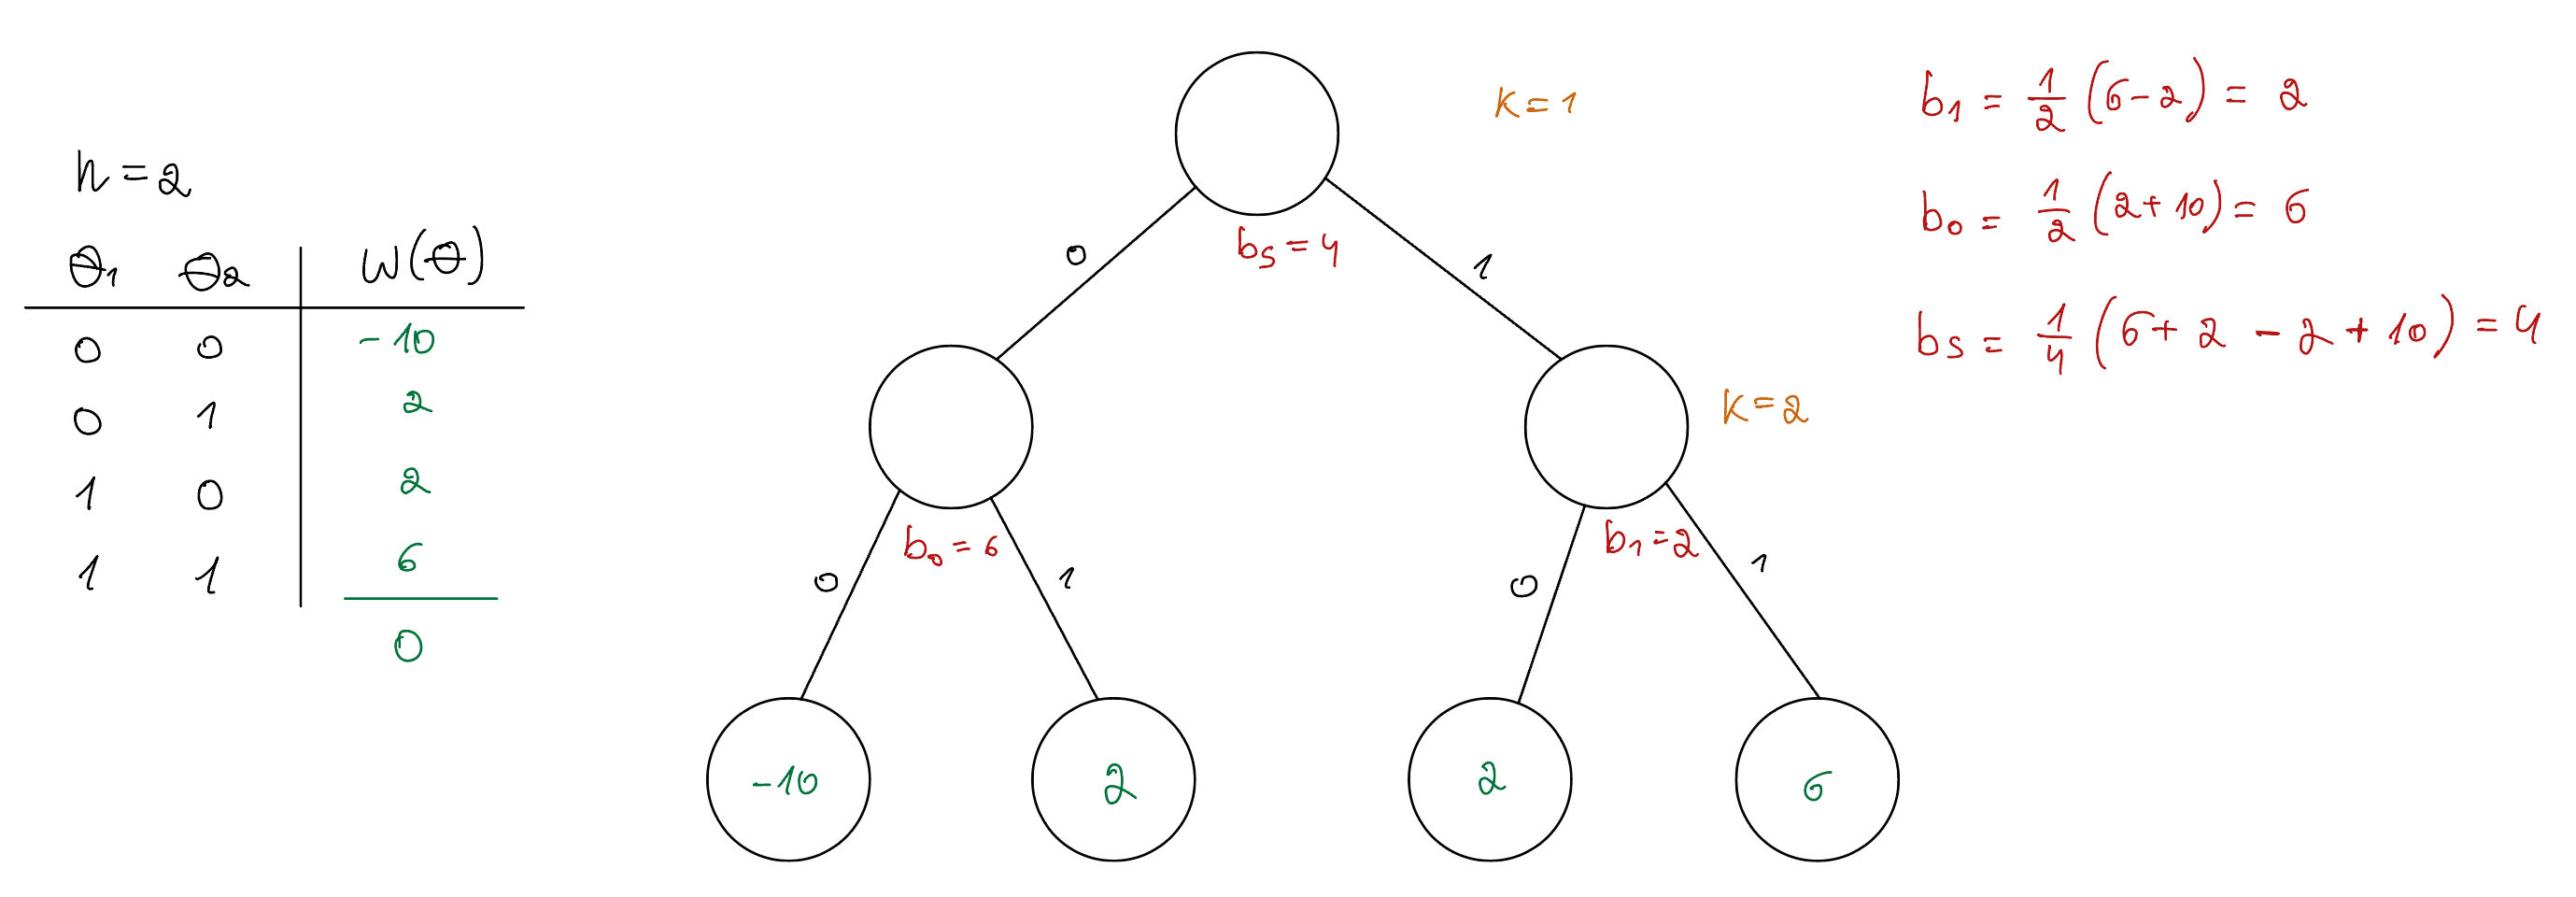
\includegraphics[width=\textwidth]{figs/achievable_winning.jpeg}
    \caption{Sequential Betting Scheme}
\end{figure}


\bigbreak

\textbf{Summary:}

Consider a betting strategy for a game against sequences: $\Theta = (\Theta_1, \Theta_2, \ldots, \Theta_n) \in \{0,1\}^n$, which allows the bet $b_k$ at stage $k$ to be some 
element in a subset $B_k$ of the collection $B$ of all functions from $\{0,1\}^n$ to $\mathbb{R}$. 
Let $w: \{0,1\}^n \rightarrow \mathbb{R}$ be a desired set of net winnings defined for each sequence $\Theta$ in $\{0,1\}^n$. 
As before, \ref{eq:3.1} expresses the net winnings $w(\Theta)$ as a function of $\{b_1, b_2, \ldots, b_n\}$. Then:

\begin{enumerate}
    \item[(II)] Trivially, if $B_k = B$, any $w$ is achievable.
    \item[(III)] If $B_k$ is the set of all functions in $B$ depending only on $\Theta_1, \Theta_2, \ldots, \Theta_{k-1}$, then $w$ is achievable if and only if $(3.5)$ is satisfied.
    \item[(IV)] If, for $k = 1, 2, \ldots, n$, $B_k \subseteq B$ is the set of functions bounded in absolute value by $b$, depending only on $\Theta_1, \Theta_2, \ldots, \Theta_{k-1}$, 
    then $w$ is achievable if and only if
    \begin{align} \label{eq:3.7}
        \sum_{\Theta} w(\Theta) &= 0 
    \end{align}
    and if, for $k = 1, 2, \ldots, n$,
    \begin{align} \label{eq:3.8}
        \left|\left(\frac{1}{2}\right)^{n-k+1} \sum_{(\Theta_k, \Theta_{k+1}, \ldots, \Theta_n) \in \{0,1\}^{n-k+1}} w(\Theta)(2\Theta_k - 1)\right| &< b 
    \end{align}
    for every $(\Theta_1, \Theta_2, \ldots, \Theta_{k-1}) \in \{0, 1\}^{k-1}$. This is the sequential betting scheme with bounded bet size.
\end{enumerate}


% * * * * * * * * * * * * * * * * * * * * * * * * 
% * * * * * * * * * * * * * * * * * * * * * * * * 
% * * * * * * * * * * * * * * * * * * * * * * * * 
% * * * * * * * * * * * * * * * * * * * * * * * * 
% * * * * * * * * * * * * * * * * * * * * * * * * 
\subsection{Winnings which are functions of $\sum_{i=1}^{n} \Theta_i$}


We may be interested in winnings $w$ which are functions only of $\sum_{i=1}^n \Theta_i$, the number of $1$'s in $\Theta$. In this case, define, for every $\Theta \in \{0, 1\}^n$,
\begin{equation} \label{eq:3.9}
    \hat{w} \left(\sum_{i=1}^n \Theta_i\right) = w(\Theta).
\end{equation}

Then the conditions of \ref{eq:3.7} and \ref{eq:3.8} become respectively
\begin{equation} \label{eq:3.10}
    \sum_{k=0}^n \binom{n}{k} \hat{w}(k) = 0
\end{equation}
and
\begin{equation} \label{eq:3.11}
    \left|b_k(i)\right| = \left|\left(\frac{1}{2}\right)^{n-k+1} \sum_{j=0}^{n-k} \left(\hat{w}(i+j+1) - \hat{w}(i+j)\right) \binom{n-k}{j}\right| < b
\end{equation}

For \(i = 0, 1, \ldots, k - 1\) and \(k = 1, 2, \ldots, n\) where
$b_k(i)$ is the bet at stage \(k\) when the sum of the first \(k - 1\) outcomes is \(i\).

Letting \(k = n\) in (3.11) we have the condition:
\begin{equation} \label{eq:3.12}
    \left |b_n(i) \right| = \frac{1}{2} \left| \hat{w}(i + 1) - \hat{w}(i)\right| < b
\end{equation}
for \(i = 0, 1, \ldots, n - 1\).

All other conditions of (3.11) are consequences of (3.12), since, assuming (3.12) true,
\begin{equation} \label{eq:3.13}
    \begin{aligned}
        \left|b_k(i)\right| &= \left| \left(\frac{1}{2}\right)^{n-k+1} \sum_{j=0}^{n-k} \left(w(i + j + 1) - w(i + j)\right) \binom{n-k}{j} \right| \leq \\
        &\left(\frac{1}{2}\right)^{n-k+1} \sum_{j=0}^{n-k} \binom{n-k}{j} 2b = b.
    \end{aligned}
\end{equation}

Hence, a terminal score \(\hat{w}\) depending only on \(\sum_{i=1}^n \Theta_i\) is achievable by a sequential betting scheme with bounded bet size \(b\) if and only if
\begin{equation} \label{eq:3.14}
    \sum_{k=0}^n \binom{n}{k} \hat{w}(k) = 0
\end{equation}
and
\begin{equation} \label{eq:3.15}
    \left| \hat{w}(k + 1) - \hat{w}(k)\right| < 2b, \quad k = 1, 2, \ldots, n - 1.
\end{equation}

% * * * * * * * * * * * * * * * * * * * * * * * * 
% * * * * * * * * * * * * * * * * * * * * * * * * 
% * * * * * * * * * * * * * * * * * * * * * * * * 
% * * * * * * * * * * * * * * * * * * * * * * * * 
% * * * * * * * * * * * * * * * * * * * * * * * * 
\subsection{Examples}

\subsubsection{Example 1 - foreknowledge of a sequence which will not occur}

Consider a gambler betting on a binary sequence of length \(n\), consisting of 1's and 0's. 
The gambler can choose his bet amount at each stage, based on the sequence observed so far. 
Suppose the gambler knows in advance that a specific sequence, say \(\Theta^*\), will not occur. 
The question is whether the gambler can guarantee a profit. The answer is yes; he can potentially win an infinite amount. 

For any goal function \(w(\Theta)\), there exists a betting strategy that guarantees a win of \(w(\Theta)\) 
for any sequence \(\Theta \neq \Theta^*\). This is achieved by setting:
\[
w(\Theta^*) = -\sum_{\Theta \neq \Theta^*} w(\Theta)
\]
and applying the betting strategy outlined in section \(3.6\).
This example illustrates that, under certain conditions, a gambler can manipulate his bets based on a probability distribution over possible outcomes 
to achieve a desired terminal wealth distribution. 

\subsubsection{Example 2 - independent flips of a fair coin}


Let \(\Theta_1, \cdots, \Theta_n\) be independent flips of a fair coin. 
For a desired distribution function \( F \), there exists a sequential betting scheme achieving a terminal distribution \( F_n \) such that 
\[
\sup_x |F(x) - F_n(x)| < \frac{1}{2^n}
\]

To achieve $F_n$ in the case of continuous $F$, choose $w_i$ such that $F(w_i) = \frac{i}{2^n}$ for $i = 1, 2, \ldots, 2^n - 1$ and $w_0 = -\sum_{i=1}^{2^n - 1} w_i$.
Associate the winnings $w$ with the outcomes $\Theta$'s in an arbitrary fashion and use the betting scheme of \ref{eq:3.6}.


\subsection{Summary}

Our investigations reveal that while almost any probability distribution for terminal capital can theoretically be achieved through sequential 
betting strategies, in practice, most terminal distributions are not appealing to gamblers. 
This disinterest largely stems from the nature of popular gambling systems like Martingale and Progression Systems, 
which typically offer small gains offset by a significant risk of substantial losses.

Most betting systems fail to optimize gambler's utilities because they do not sufficiently reward the risk of extreme outcomes, 
leading to inherently suboptimal strategies. The utility functions, if properly utilized to influence betting decisions, 
should account for the potential gains at the extremes of the distribution. However, the increase at a few terminal points, 
as suggested by theoretical models, often does not compensate for the overall risk, making these strategies less favorable.




% * * * * * * * * * * * * * * * * * * * * * * * * 
% * * * * * * * * * * * * * * * * * * * * * * * * 
% * * * * * * * * * * * * * * * * * * * * * * * * 
% * * * * * * * * * * * * * * * * * * * * * * * * 
% * * * * * * * * * * * * * * * * * * * * * * * * 
% * * * * * * * * * * * * * * * * * * * * * * * * 
% * * * * * * * * * * * * * * * * * * * * * * * * 
% * * * * * * * * * * * * * * * * * * * * * * * * 
% * * * * * * * * * * * * * * * * * * * * * * * * 
% * * * * * * * * * * * * * * * * * * * * * * * * 
% * * * * * * * * * * * * * * * * * * * * * * * * 
% * * * * * * * * * * * * * * * * * * * * * * * * 
% * * * * * * * * * * * * * * * * * * * * * * * * 
% * * * * * * * * * * * * * * * * * * * * * * * * 
% * * * * * * * * * * * * * * * * * * * * * * * * 
% * * * * * * * * * * * * * * * * * * * * * * * * 
% * * * * * * * * * * * * * * * * * * * * * * * * 
% * * * * * * * * * * * * * * * * * * * * * * * * 
% * * * * * * * * * * * * * * * * * * * * * * * * 
\section{Random Predictors}





% * * * * * * * * * * * * * * * * * * * * * * * * 
% * * * * * * * * * * * * * * * * * * * * * * * * 
% * * * * * * * * * * * * * * * * * * * * * * * * 
% * * * * * * * * * * * * * * * * * * * * * * * * 
% * * * * * * * * * * * * * * * * * * * * * * * * 
% * * * * * * * * * * * * * * * * * * * * * * * * 
% * * * * * * * * * * * * * * * * * * * * * * * * 
% * * * * * * * * * * * * * * * * * * * * * * * * 
% * * * * * * * * * * * * * * * * * * * * * * * * 
% * * * * * * * * * * * * * * * * * * * * * * * * 
% * * * * * * * * * * * * * * * * * * * * * * * * 
% * * * * * * * * * * * * * * * * * * * * * * * * 
% * * * * * * * * * * * * * * * * * * * * * * * * 
% * * * * * * * * * * * * * * * * * * * * * * * * 
% * * * * * * * * * * * * * * * * * * * * * * * * 
% * * * * * * * * * * * * * * * * * * * * * * * * 
% * * * * * * * * * * * * * * * * * * * * * * * * 
% * * * * * * * * * * * * * * * * * * * * * * * * 
% * * * * * * * * * * * * * * * * * * * * * * * * 
\section{Conclusions}




\end{document}